%File: anonymous-submission-latex-2025.tex
\documentclass[letterpaper]{article} % DO NOT CHANGE THIS

\usepackage[submission]{aaai25}  % DO NOT CHANGE THIS
\usepackage{times}  % DO NOT CHANGE THIS
\usepackage{helvet}  % DO NOT CHANGE THIS
\usepackage{courier}  % DO NOT CHANGE THIS
\usepackage[hyphens]{url}  % DO NOT CHANGE THIS
\usepackage{graphicx} % DO NOT CHANGE THIS
\urlstyle{rm} % DO NOT CHANGE THIS
\def\UrlFont{\rm}  % DO NOT CHANGE THIS
\usepackage{natbib}  % DO NOT CHANGE THIS AND DO NOT ADD ANY OPTIONS TO IT
\usepackage{caption} % DO NOT CHANGE THIS AND DO NOT ADD ANY OPTIONS TO IT
\frenchspacing  % DO NOT CHANGE THIS
\setlength{\pdfpagewidth}{8.5in} % DO NOT CHANGE THIS
\setlength{\pdfpageheight}{11in} % DO NOT CHANGE THIS
%
% These are recommended to typeset algorithms but not required. See the subsubsection on algorithms. Remove them if you don't have algorithms in your paper.
\usepackage{algorithm}
\usepackage{algorithmic}
\usepackage{amsmath}
\usepackage{amsfonts}
\usepackage{amsthm}
\usepackage{mathrsfs}
\usepackage{mathtools}
\usepackage{booktabs}
\usepackage{lipsum}
\usepackage{listings}
\usepackage[acronym]{glossaries}
\usepackage{xspace}
\usepackage{circledsteps}
\usepackage{tikz}
\usetikzlibrary{arrows.meta, calc, positioning}
\tikzset{>=latex} % for LaTeX arrow head
\usepackage{pgfplots} % for the axis environment
\usepgfplotslibrary{fillbetween} % to fill an area under function
% define gaussian pdf and cdf
\pgfmathdeclarefunction{gauss}{3}{%
    \pgfmathparse{1/(#3*sqrt(2*pi))*exp(-((#1-#2)^2)/(2*#3^2))}%
}
\usepackage[outline]{contour} % halo around text
\usetikzlibrary{patterns}
\pgfplotsset{compat=1.12} % TikZ coordinates <-> axes coordinates
% https://tex.stackexchange.com/questions/240642/add-vertical-line-of-equation-x-2-and-shade-a-region-in-graph-by-pgfplots

\usepackage{environ}
\usepackage{import}
\usepackage{pgf}
\usepackage{comment}
\DeclareCaptionStyle{ruled}{labelfont=normalfont,labelsep=colon,strut=off}
% \lstset{%
%     basicstyle={\footnotesize\ttfamily},% footnotesize acceptable for monospace
%     numbers=left,numberstyle=\footnotesize,xleftmargin=2em,% show line numbers, remove this entire line if you don't want the numbers.
%     aboveskip=2pt,
%     belowskip=2pt,
%     showstringspaces=false,
%     tabsize=2,
%     breaklines=true}
\usepackage{xcolor}
\newcommand{\Sadegh}{\textcolor{magenta}}

% Resolve problems with .eps figures
\usepackage{graphicx}
\usepackage[outdir=./]{epstopdf}
\graphicspath{{./figures/}} %Where the figures folder is located

% Include check and cross marks for qualitative comparison table
\usepackage{pifont}% http://ctan.org/pkg/pifont
\newcommand{\cmark}{\ding{51}} % Checkmark
\newcommand{\xmark}{\ding{55}} % X-mark
\newcommand{\xmarkred}{{\color{magenta}\xmark}} % Red colored X-mark
\definecolor{accent}{RGB}{160,32,240}
\definecolor{accent2}{RGB}{0,141,225}

% TKpicture
\usetikzlibrary{shapes.geometric, arrows.meta, positioning, fit, shadows} % Tikz library for arrows

% Common terms
\newcommand{\hp}{hyperparameters\xspace}

% Files
\newcommand{\yaml}{\textit{.yaml}\xspace}
\newcommand{\json}{\textit{.json}\xspace}

% Maths
\newcommand{\cdotx}{\,\cdot\,} % Function argument
\newcommand{\data}{\boldsymbol{\mathcal{D}}} % Data
\renewcommand{\S}{\boldsymbol{\mathcal{S}}} % System
\newcommand{\LS}{\boldsymbol{\mathcal{L}}} % Linear system
\newcommand{\BS}{\boldsymbol{\mathcal{B}}} % Barrier3
\newcommand{\T}{^\top}
\newcommand{\R}{\mathbb{R}}
\newcommand{\Z}{\mathbb{Z}}
\newcommand{\N}{\mathbb{N}}
\newcommand{\X}{\mathbb{X}}
\newcommand{\Y}{\mathbb{Y}}
\newcommand{\borel}[1]{\mathcal{B}(#1)}
\renewcommand{\P}{\mathbb{P}}
\renewcommand{\mid}{\,|\,}
\newcommand{\E}{\mathbb{E}}
\newcommand{\Q}{\mathbb{Q}}
\newcommand{\1}{\mathbbm{1}}
\newcommand{\e}{\mathbbm{e}}
\newcommand{\x}{\boldsymbol{x}}
\newcommand{\y}{\boldsymbol{y}}
\newcommand{\z}{\boldsymbol{z}}
\DeclareMathOperator{\diag}{diag}
\newcommand{\U}{\boldsymbol{U}}
\newcommand{\G}{\boldsymbol{G}}
\newcommand{\A}{\mathbb{A}}
\newcommand{\B}{\boldsymbol{B}}
\newcommand{\Hilbert}{\mathcal{H}} % Hilbert space
\newcommand{\norm}[1]{\left|\left|#1\right|\right|}
\newcommand{\I}{\boldsymbol{I}}
\newcommand{\innerH}[3]{\langle #1, #2 \rangle_{#3}} % Inner product
\newcommand{\M}{\mathbf{M}}
\newcommand{\cme}{\Psi} % Conditional mean embedding
\newcommand{\Tr}{\mathbf{t}}
\newcommand{\W}{\mathbb{W}}

% Tool names
\newcommand{\deepsplit}{\textsc{DEEPSPLIT}\xspace}
\newcommand{\fossil}{\textsc{Fossil}\xspace}
\newcommand{\lucid}{\textsc{Lucid}\xspace}
\newcommand{\pylucid}{\textsc{PyLucid}\xspace}
\newcommand{\npinterval}{\textsc{npinterval}\xspace}
\newcommand{\reluplex}{\textsc{Reluplex}\xspace}
\newcommand{\trust}{\textsc{TRUST}\xspace}
\newcommand{\gurobi}{\textsc{Gurobi}\xspace}
\newcommand{\alglib}{\textsc{Alglib}\xspace}
\newcommand{\highs}{\textsc{HiGHS}\xspace}
\newcommand{\dreal}{\textsc{dReal}\xspace}
\newcommand{\omnisafe}{\textsc{OmniSafe}\xspace}
\newcommand{\barr}{\texttt{Barr\textsubscript{3}}\xspace}

% Components
\newcommand{\estimator}{\texttt{Estimator}\xspace}

%%%%%%%%%%%%%%%%%%%%%%%%
% Theorems and co.
%%%%%%%%%%%%%%%%%%%%%%%%
\theoremstyle{definition}
\newtheorem{definition}{Definition}[section]
\theoremstyle{plain}
\newtheorem{theorem}{Theorem}[section]
\newtheorem{lemma}[theorem]{Lemma}
\newtheorem{corollary}[theorem]{Corollary}
\newtheorem{proposition}[theorem]{Proposition}
\theoremstyle{remark}
\newtheorem{remark}{Remark}[section]
\newtheorem{example}{Example}[section]
\newtheorem{assumption}{Assumption}[section]
\newtheorem{problem}{Problem}[section]
\newtheorem{claim}{Claim}[section]

% Styling
%% Python definition (c) 1998 Michael Weber
%% Additional definitions (2013) Alexis Dimitriadis
%% modified by me (should not have empty lines)
%%
\lstdefinelanguage{iPython}{
basicstyle={\footnotesize\ttfamily},% footnotesize acceptable for monospace
numbers=left,numberstyle=\footnotesize,xleftmargin=2em,% show line numbers, remove this entire line if you don't want the numbers.
aboveskip=2pt,
belowskip=2pt,
showstringspaces=false,
tabsize=2,
breaklines=true,
morekeywords={as,access,and,break,class,continue,def,del,elif,else,except,exec,finally,for,from,global,if,import,in,is,lambda,not,or,pass,print,raise,return,try,while},%
%
% Built-ins
morekeywords=[2]{abs,all,any,basestring,bin,bool,bytearray,callable,chr,classmethod,cmp,compile,complex,delattr,dict,dir,divmod,enumerate,eval,execfile,file,filter,float,format,frozenset,getattr,globals,hasattr,hash,help,hex,id,input,int,isinstance,issubclass,iter,len,list,locals,long,map,max,memoryview,min,next,object,oct,open,ord,pow,property,range,raw_input,reduce,reload,repr,reversed,round,set,setattr,slice,sorted,staticmethod,str,sum,super,tuple,type,unichr,unicode,vars,xrange,zip,apply,buffer,coerce,intern},%
%
sensitive=true,%
morecomment=[l]\#,%
morestring=[b]',%
morestring=[b]",%
%
morestring=[s]{'''}{'''},% used for documentation text (mulitiline strings)
morestring=[s]{"""}{"""},% added by Philipp Matthias Hahn
%
morestring=[s]{r'}{'},% `raw' strings
morestring=[s]{r"}{"},%
morestring=[s]{r'''}{'''},%
morestring=[s]{r"""}{"""},%
morestring=[s]{u'}{'},% unicode strings
morestring=[s]{u"}{"},%
morestring=[s]{u'''}{'''},%
morestring=[s]{u"""}{"""},%
%
% {replace}{replacement}{lenght of replace}
% *{-}{-}{1} will not replace in comments and so on
literate=
    *{+}{{{\color{ipython_purple}+}}}1
{-}{{{\color{ipython_purple}-}}}1
{*}{{{\color{ipython_purple}$^\ast$}}}1
{/}{{{\color{ipython_purple}/}}}1
{^}{{{\color{ipython_purple}\^{}}}}1
{?}{{{\color{ipython_purple}?}}}1
{!}{{{\color{ipython_purple}!}}}1
{\%}{{{\color{ipython_purple}\%}}}1
{<}{{{\color{ipython_purple}<}}}1
{>}{{{\color{ipython_purple}>}}}1
{|}{{{\color{ipython_purple}|}}}1
{\&}{{{\color{ipython_purple}\&}}}1
{~}{{{\color{ipython_purple}~}}}1
%
{==}{{{\color{ipython_purple}==}}}2
{<=}{{{\color{ipython_purple}<=}}}2
{>=}{{{\color{ipython_purple}>=}}}2
%
{+=}{{{+=}}}2
{-=}{{{-=}}}2
{*=}{{{$^\ast$=}}}2
{/=}{{{/=}}}2,
%
literate=
    {á}{{\'a}}1 {é}{{\'e}}1 {í}{{\'i}}1 {ó}{{\'o}}1 {ú}{{\'u}}1
{Á}{{\'A}}1 {É}{{\'E}}1 {Í}{{\'I}}1 {Ó}{{\'O}}1 {Ú}{{\'U}}1
{à}{{\`a}}1 {è}{{\`e}}1 {ì}{{\`i}}1 {ò}{{\`o}}1 {ù}{{\`u}}1
{À}{{\`A}}1 {È}{{\'E}}1 {Ì}{{\`I}}1 {Ò}{{\`O}}1 {Ù}{{\`U}}1
{ä}{{\"a}}1 {ë}{{\"e}}1 {ï}{{\"i}}1 {ö}{{\"o}}1 {ü}{{\"u}}1
{Ä}{{\"A}}1 {Ë}{{\"E}}1 {Ï}{{\"I}}1 {Ö}{{\"O}}1 {Ü}{{\"U}}1
{â}{{\^a}}1 {ê}{{\^e}}1 {î}{{\^i}}1 {ô}{{\^o}}1 {û}{{\^u}}1
{Â}{{\^A}}1 {Ê}{{\^E}}1 {Î}{{\^I}}1 {Ô}{{\^O}}1 {Û}{{\^U}}1
{œ}{{\oe}}1 {Œ}{{\OE}}1 {æ}{{\ae}}1 {Æ}{{\AE}}1 {ß}{{\ss}}1
{ç}{{\c c}}1 {Ç}{{\c C}}1 {ø}{{\o}}1 {å}{{\r a}}1 {Å}{{\r A}}1
{€}{{\EUR}}1 {£}{{\pounds}}1,
%
%   identifierstyle=\color{red}\ttfamily,
commentstyle=\color{ipython_cyan}\ttfamily,
stringstyle=\color{ipython_red}\ttfamily,
keepspaces=true,
showspaces=false,
%
rulecolor=\color{ipython_frame},
%
%
numberstyle=\tiny\color{halfgray},
backgroundcolor=\color{ipython_bg},
%   extendedchars=true,
keywordstyle=\color{ipython_green}\ttfamily,
}
\lstdefinelanguage{yaml}{
numbers=none,
xleftmargin=0em,
keywords = {true,false,null,y,n},
sensitive=false,
comment=[l]{\#},
morecomment=[s]{/*}{*/},
commentstyle=\color{commentGreen}\ttfamily,
stringstyle=\color{stringRed}\ttfamily,
keywordstyle=\color{keywordBlue}\bfseries,
moredelim=**[il][\color{commentGreen}{:}\color{keywordBlue}]{:},
morestring=[b]",
morestring=[b]',
literate =  {---}{{\ProcessThreeDashes}}3
{>}{{\textcolor{red}\textgreater}}1
{|}{{\textcolor{red}\textbar}}1
{\ -\ }{{\mdseries\ -\ }}3,
}

\definecolor{commentGreen}{RGB}{0, 100, 0}
\definecolor{stringRed}{RGB}{163, 21, 21}
\definecolor{keywordBlue}{RGB}{0, 0, 255}

% Colors
\definecolor{halfgray}{gray}{0.55}
\definecolor{ipython_frame}{RGB}{207, 207, 207}
\definecolor{ipython_bg}{RGB}{247, 247, 247}
\definecolor{ipython_red}{RGB}{186, 33, 33}
\definecolor{ipython_green}{RGB}{0, 128, 0}
\definecolor{ipython_cyan}{RGB}{64, 128, 128}
\definecolor{ipython_purple}{RGB}{170, 34, 255}

% Other
\newcommand{\todo}[1]{\textcolor{purple}{\textbf{TODO}: \textit{#1}}}
\newcommand{\new}[1]{#1}
\newcommand{\OS}[1]{{\color{blue}[Oliver]: #1}}
\newcommand{\EC}[1]{{\color{brown}[Ernesto]: #1}}

% These are are recommended to typeset listings but not required. See the subsubsection on listing. Remove this block if you don't have listings in your paper.
\usepackage{newfloat}
\usepackage{listings}
\DeclareCaptionStyle{ruled}{labelfont=normalfont,labelsep=colon,strut=off} % DO NOT CHANGE THIS
\lstset{%
    basicstyle={\footnotesize\ttfamily},% footnotesize acceptable for monospace
    numbers=left,numberstyle=\footnotesize,xleftmargin=2em,% show line numbers, remove this entire line if you don't want the numbers.
    aboveskip=2pt,belowskip=2pt,%
    showstringspaces=false,tabsize=2,breaklines=true}
\floatstyle{ruled}
\newfloat{listing}{tb}{lst}{}
\floatname{listing}{Listing}
\lstdefinestyle{nonumbers}{numbers=none,numberstyle=\footnotesize,xleftmargin=0em}
%
% Keep the \pdfinfo as shown here. There's no need
% for you to add the /Title and /Author tags.
\pdfinfo{
    /TemplateVersion (2025.1)
}

% DISALLOWED PACKAGES
% \usepackage{authblk} -- This package is specifically forbidden
% \usepackage{balance} -- This package is specifically forbidden
% \usepackage{color (if used in text)
% \usepackage{CJK} -- This package is specifically forbidden
% \usepackage{float} -- This package is specifically forbidden
% \usepackage{flushend} -- This package is specifically forbidden
% \usepackage{fontenc} -- This package is specifically forbidden
% \usepackage{fullpage} -- This package is specifically forbidden
% \usepackage{geometry} -- This package is specifically forbidden
% \usepackage{grffile} -- This package is specifically forbidden
% \usepackage{hyperref} -- This package is specifically forbidden
% \usepackage{navigator} -- This package is specifically forbidden
% (or any other package that embeds links such as navigator or hyperref)
% \indentfirst} -- This package is specifically forbidden
% \layout} -- This package is specifically forbidden
% \multicol} -- This package is specifically forbidden
% \nameref} -- This package is specifically forbidden
% \usepackage{savetrees} -- This package is specifically forbidden
% \usepackage{setspace} -- This package is specifically forbidden
% \usepackage{stfloats} -- This package is specifically forbidden
% \usepackage{tabu} -- This package is specifically forbidden
% \usepackage{titlesec} -- This package is specifically forbidden
% \usepackage{tocbibind} -- This package is specifically forbidden
% \usepackage{ulem} -- This package is specifically forbidden
% \usepackage{wrapfig} -- This package is specifically forbidden
% DISALLOWED COMMANDS
% \nocopyright -- Your paper will not be published if you use this command
% \addtolength -- This command may not be used
% \balance -- This command may not be used
% \baselinestretch -- Your paper will not be published if you use this command
% \clearpage -- No page breaks of any kind may be used for the final version of your paper
% \columnsep -- This command may not be used
% \newpage -- No page breaks of any kind may be used for the final version of your paper
% \pagebreak -- No page breaks of any kind may be used for the final version of your paperr
% \pagestyle -- This command may not be used
% \tiny -- This is not an acceptable font size.
% \vspace{- -- No negative value may be used in proximity of a caption, figure, table, section, subsection, subsubsection, or reference
% \vskip{- -- No negative value may be used to alter spacing above or below a caption, figure, table, section, subsection, subsubsection, or reference

\setcounter{secnumdepth}{2} %May be changed to 1 or 2 if section numbers are desired.

% The file aaai25.sty is the style file for AAAI Press
% proceedings, working notes, and technical reports.
%

%%%%%%%%%%%%%%%%%%%%%%%%
% Glossary
%%%%%%%%%%%%%%%%%%%%%%%%
\glsdisablehyper
\input{glossary.tex}
% \makeglossaries
% \loadglsentries{glossary}


%%%%%%% Include tikz document shape %%%%%%%
% taken from manual
\makeatletter
\pgfdeclareshape{document}{
    \inheritsavedanchors[from=rectangle] % this is nearly a rectangle
    \inheritanchorborder[from=rectangle]
    \inheritanchor[from=rectangle]{center}
    \inheritanchor[from=rectangle]{north}
    \inheritanchor[from=rectangle]{south}
    \inheritanchor[from=rectangle]{west}
    \inheritanchor[from=rectangle]{east}
    % ... and possibly more
    \backgroundpath{% this is new
        % store lower right in xa/ya and upper right in xb/yb
        \southwest \pgf@xa=\pgf@x \pgf@ya=\pgf@y
        \northeast \pgf@xb=\pgf@x \pgf@yb=\pgf@y
        % compute corner of ‘‘flipped page’’
        \pgf@xc=\pgf@xb \advance\pgf@xc by-10pt % this should be a parameter
        \pgf@yc=\pgf@yb \advance\pgf@yc by-10pt
        % construct main path
        \pgfpathmoveto{\pgfpoint{\pgf@xa}{\pgf@ya}}
        \pgfpathlineto{\pgfpoint{\pgf@xa}{\pgf@yb}}
        \pgfpathlineto{\pgfpoint{\pgf@xc}{\pgf@yb}}
        \pgfpathlineto{\pgfpoint{\pgf@xb}{\pgf@yc}}
        \pgfpathlineto{\pgfpoint{\pgf@xb}{\pgf@ya}}
        \pgfpathclose
        % add little corner
        \pgfpathmoveto{\pgfpoint{\pgf@xc}{\pgf@yb}}
        \pgfpathlineto{\pgfpoint{\pgf@xc}{\pgf@yc}}
        \pgfpathlineto{\pgfpoint{\pgf@xb}{\pgf@yc}}
        \pgfpathlineto{\pgfpoint{\pgf@xc}{\pgf@yc}}
    }
}
\makeatother
%%%%%%%%%%%%%%%%%%%%%%%%%%%%%%%%%%%

% Title

% Your title must be in mixed case, not sentence case.
% That means all verbs (including short verbs like be, is, using,and go),
% nouns, adverbs, adjectives should be capitalized, including both words in hyphenated terms, while
% articles, conjunctions, and prepositions are lower case unless they
% directly follow a colon or long dash
\title{LUCID: Learning-Enabled Uncertainty-Aware Certification of Stochastic Dynamical Systems}
%\title{LUCID -- ???}
% Black-Box Verification Engine for Embodied AI Systems?
% \author {
%     % Authors
    % Ernesto Casablanca\textsuperscript{\rm 1},
    % Oliver Sch\"on\textsuperscript{\rm 1}%,
    % Third Author Name\textsuperscript{\rm 2}
% }
% \affiliations {
    % Affiliations
    % \textsuperscript{\rm 1}Newcastle University, United Kingdom\\
    % \textsuperscript{\rm 2}Affiliation 2\\
    % e.casablanca2@ncl.ac.uk, o.schoen2@ncl.ac.uk%, thirdAuthor@affiliation1.com
% }


% REMOVE THIS: bibentry
% This is only needed to show inline citations in the guidelines document. You should not need it and can safely delete it.
\usepackage{bibentry}
% END REMOVE bibentry

\begin{document}

\maketitle

\begin{abstract}
    Ensuring the safety of AI-enabled systems, particularly in high-stakes domains such as autonomous driving and healthcare, has become increasingly critical.
    Traditional formal verification tools fall short when faced with systems that embed both opaque, black-box AI components and complex stochastic dynamics.
    To address these challenges, we introduce \lucid (Learning-enabled Uncertainty-aware Certification of stochastIc Dynamical systems), a verification engine for certifying safety of black-box stochastic dynamical systems from a finite dataset of random state transitions.
    As such, \lucid is the first known tool capable of establishing quantified safety guarantees for such systems.
    Thanks to its modular architecture and extensive documentation, \lucid is designed for easy extensibility.

    \lucid employs a data-driven methodology rooted in control barrier certificates, which are learned directly from system transition data, to ensure formal safety guarantees.
    We use conditional mean embeddings to embed data into a reproducing kernel Hilbert space (RKHS), where an RKHS ambiguity set is constructed that can be inflated to robustify the result to out-of-distribution behavior.
    
    A key innovation within \lucid is its use of a finite Fourier kernel expansion to reformulate a semi-infinite non-convex optimization problem into a tractable linear program.
    The resulting spectral barrier allows us to leverage the fast Fourier transform to generate the relaxed problem efficiently, offering a scalable yet distributionally robust framework for verifying safety.
    \lucid thus offers a robust and efficient verification framework, able to handle the complexities of modern black-box systems while providing formal guarantees of safety.
    These unique capabilities are demonstrated on challenging benchmarks. 
\end{abstract}

% Uncomment the following to link to your code, datasets, an extended version or similar.
%
\begin{links}
    \link{Anonymized Code}{https://google.com \Sadegh{Add the link to the repo}}
    % \link{Code}{https://aaai.org/example/code}
    % \link{Datasets}{https://aaai.org/example/datasets}
    % \link{Extended version}{https://aaai.org/example/extended-version}
\end{links}
%%%%%%%%%%%%%%%%%%%%%%%%%%%%%%%%%%%%%%%%%%%%
%%%%%%%%%%%%%%%%%%%%%%%%%%%%%%%%%%%%%%%%%%%%
%%%%%%%%%%%%%%%%%%%%%%%%%%%%%%%%%%%%%%%%%%%%


\section{Introduction}
\todo{Motivation and background ...}

Trustworthy embodied AI: AI agency in physical world

Whilst verification tools for e.g. neural networks rely on the availability of the neural network model, for closed-loop systems such models are often not available or simulators are much too complicated to perform verification on directly.

% \lipsum[1-3]

\begin{table}
    \centering
    \begin{tabular}{ccccccc}
        \toprule
        \textbf{Tool}                                    & \multicolumn{6}{c}{\textbf{Supported Features}}                                                                                                                               \\[.4em]
                                                         & \rotatebox{90}{Guarantees} & \rotatebox{90}{Data Driven}                     & \rotatebox{90}{Stochastic D.} & \rotatebox{90}{Non-Poly. D.} & \rotatebox{90}{Stat. Correct.} & \rotatebox{90}{Closed Loop} \\
        \midrule
        \textbf{\lucid}& \cmark                                  & \cmark                                          & \cmark                        & \cmark                       & \cmark                              & \cmark                      \\
        \trust~\shortcite{gardner2025trust}& \cmark              & \cmark                                          & \xmarkred                     & \xmarkred                    & \cmark\footnotemark            & \cmark                      \\
        \fossil~\shortcite{edwards2024fossil}& \cmark            & \xmarkred                                       & \xmarkred                     & \cmark                       & NA                             & \cmark                      \\
        \omnisafe~\shortcite{ji2024omnisafe} & \xmarkred                                            &        \cmark                                         &        \cmark                       &                 \cmark             &          \xmarkred                            &   \cmark                     \\
        \npinterval~\shortcite{harapanahalli2023forward}& \cmark & \xmarkred                                       & \cmark/\xmarkred\footnotemark & ?                            & NA                             & \cmark                      \\
        % \deepsplit~\shortcite{henriksen2021deepsplit} & \xmarkred & \xmarkred & \cmark & \xmarkred& \xmarkred \\
        % \reluplex~\shortcite{katz2017reluplex} & \xmarkred & \xmarkred & \cmark & \xmarkred & \xmarkred \\
        tool6                                           &                                                 &                               &                              &                                                              \\
        \bottomrule
    \end{tabular}
    \caption{Qualitative comparison with existing tools based on their supported features: quantified coverage guarantees, data driven, stochastic dynamics, non-polynomial dynamics, statistical correctness guarantees of the learned model (only applicable if data driven), and support for closed-loop systems.}
    \label{tab:qualitative_comparison}
\end{table}
\footnotetext{Assuming the data satisfies persistence of excitation.} % TRUST
\footnotetext{Accepts non-deterministic bounded disturbances.} % npinterval


\OS{Need to mention the difference between quantified coverage guarantees and statistical correctness guarantees}

The main contributions of this work are:
\begin{itemize}
    \item A novel verification engine that learns control barrier certificates from data using kernel methods and conditional mean embeddings.
    \item A tractable reformulation of the verification problem via finite Fourier expansion, enabling efficient linear programming-based synthesis of barrier certificates.
    \item A robust and extensible software implementation, with both C++ and Python interfaces, supporting configuration via YAML, JSON, or Python scripts, and offering both CLI and GUI modes.
    \item Comprehensive evaluation on a suite of benchmarks, demonstrating \lucid{}’s scalability, robustness, and practical utility.
\end{itemize}


\paragraph{Related Work (optionally)}
None of the tools provide an answer to the problem we are solving here!

Different categories for verification in annual friendly competitions~\cite{abate2024arch}.
There exist a lot of tools for verifying the input--output behavior of neural networks~\cite{liu2021algorithms}.
For closed-loop systems, ... [see literature in \cite{harapanahalli2023forward}]
Black-box verification of stochastic dynamical systems very sparsely populated.
Comparison with the most related existing tools in Table~\ref{tab:qualitative_comparison}: Focus on data-driven tools, with few exceptions if noteworthy because very related.
Result: Few data-driven tools; No data-driven tools for stochastic systems.

\citet{ji2024omnisafe} present \omnisafe, a comprehensive platform for the development of safe reinforcement learning (RL) algorithms. In comparison to \lucid, safe RL does generally only \emph{encourage} safer behavior, without providing any rigorous or quantified guarantees on the probability of the absence of any unsafe behavior.

\Sadegh{When describing Table 1, it would be good if we could also highlight the underlying major assumptions raised in any of these papers. I guess we are the ones putting the least assumption.}

What are the working principles used. 
No other kernel-based tools? (foundations of distributionally robust barrier certificates in \cite{schoen2024distributionally,chen2025distributionally} (the latter only uncertain stochastic noise), both leading to SOS-based formulations) \OS{Or rather add \cite{chen2025ontheconstruction} instead?}
Not tools: What works have achieved related things.
Sampling-based reachability analysis~\cite{lew2021sampling}.

\OS{We should make clear how the presented approach compares to conformal prediction.}

% \lipsum[1]



\paragraph{Organization}
The paper is organized as follows:
Section~\ref{sec:theory} provides the theoretical foundations of \lucid, including the safety of black-box dynamical systems, control barrier certificates, conditional mean embeddings, and linear programming.
Section~\ref{sec:tool} describes the architecture and functionalities of \lucid, including its components and how they interact.
Section~\ref{sec:example} presents a simple example use case, demonstrating how to use \lucid to certify the safety of a simple linear system.
Finally, Section~\ref{sec:experiments} evaluates \lucid on a suite of benchmarks, demonstrating its scalability, robustness, and practical utility. \Sadegh{Revise this paragraph as there is no section number.}

\section{Theoretical Working Principles}\label{sec:theory}
\subsection{Safety of Black-Box Dynamical Systems}

\paragraph{System Description}
Many AI-driven systems exhibit complex, nonlinear, and stochastic behavior that can be modeled as discrete-time stochastic processes with Markovian dynamics:
\begin{equation}
    \label{eq:model}
    \S\colon\quad x_{t+1}  = f(x_t,a_t,w_t),\quad w_t\sim p_w,
\end{equation}
where $f\colon\X\times\A\times\W\rightarrow\X$ is a continuous vector field describing the evolution of the system state $x_t\in\X\subset\R^n$ over time $t\in\N_{\geq0}$, driven by control actions $a_t\in\A\subset\R^m$ and process noise $w_t\in\W\subset\R^l$.
The noise is assumed to be drawn from a stochastic distribution $p_w$ in an independent and identically distributed (i.i.d.) manner.
%
This general formulation subsumes a wide range of systems, including discrete-time Markov decision processes (MDPs).


\paragraph{Black-Box Policies}
Here, the focus is on systems $\S$ driven by black-box control policies of the form $\pi\colon\R^n\rightarrow\R^m$, i.e., at every time step $t=0,1,2,\ldots$ a continuous action $a_t\in\A$ is selected based on the current state $x_t$. Such policies could be, for example, neural networks trained via RL, or any other black-box function generating actions in $\R^m$ (see Figure~\ref{fig:closed_loop_system}).
The resulting closed-loop system is denoted as $\S^\pi$.
\begin{figure}
    \centering
    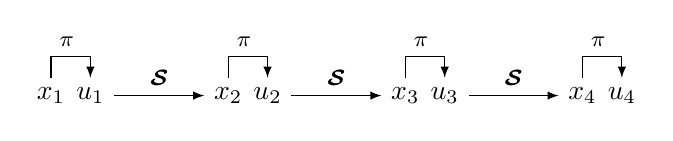
\begin{tikzpicture}
	\foreach \i in {4, ..., 1}{
		\node[name=xa\i] at (\i/4*9,0) {$x_\i$};
	}
	\foreach \i in {4, ..., 1}{
		\node[name=aa\i] at (\i/4*9+.5,0) {$u_{\i}$};
	}
	\foreach \i in {4, ..., 1}{
		\path[draw,->] (xa\i) -- +(0,.5)-| node[left,above,xshift = -0.3cm]{\footnotesize$\pi$} (aa\i);
	}
	\foreach \i in {3, ..., 1}{
		\pgfmathtruncatemacro{\j}{\i + 1}
		\path[draw,->] (aa\i)-- node[above]{\footnotesize$\S$} (xa\j);
	}
\end{tikzpicture}
    \caption{Evolution of the closed-loop system.}
    \label{fig:closed_loop_system}
\end{figure}

\paragraph{Dataset}
Due to their complexity and opacity, such systems must often be treated as black boxes in their entirety, assuming only access to a finite amount of system observations of the form
\begin{equation}
    \data_N\colon \quad \{x^i,a^i,x^i_+\}_{i=1}^N,\label{eq:data}
\end{equation}
where every sample is generated as a realization
\begin{equation*}
    (x^i,a^i,x_+^i)\sim\int \delta_{f(x^i,a^i,w)}\,p_w(dw)\,\mathcal{U}_\X(dx^i)\,\mathcal{U}_\A(da^i),
\end{equation*}
with $\mathcal{U}_\X,\mathcal{U}_\A$ uniform distributions on $\X$ and $\A$, respectively.

\begin{figure}[ht]
    \centering
    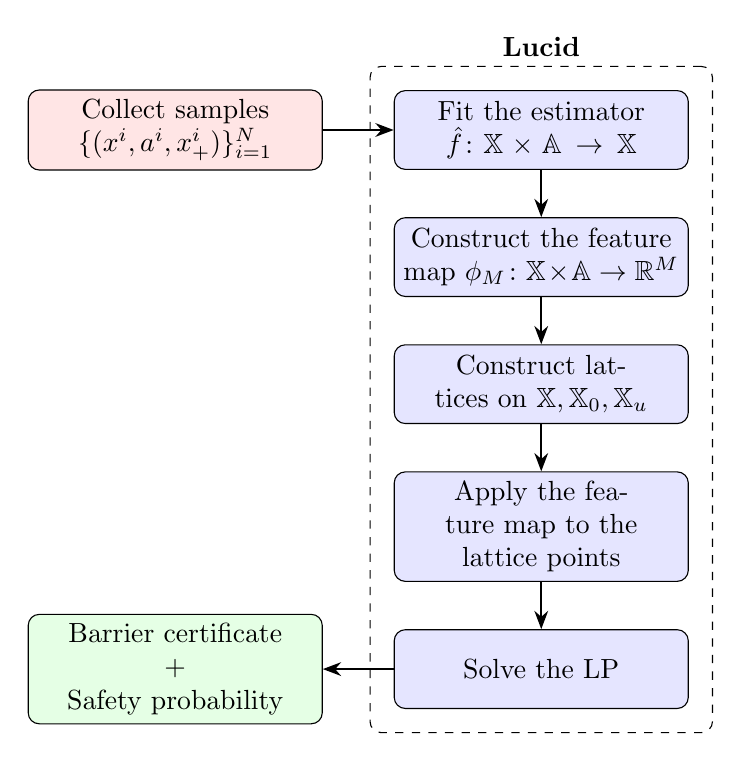
\begin{tikzpicture}[node distance=0.6cm and 0.9cm,
            input-block/.style={rectangle, draw, fill=red!10, text width=3.5cm, minimum height=1.0cm, align=center, rounded corners},
            output-block/.style={rectangle, draw, fill=green!10, text width=3.5cm, minimum height=1.0cm, align=center, rounded corners},
            block/.style={rectangle, draw, fill=blue!10, text width=3.5cm, minimum height=1.0cm, align=center, rounded corners},
            arrow/.style={thick,->,>=Stealth},
            tool/.style={rectangle, draw, fill=green!20, text width=2cm, minimum height=0.8cm, align=center, rounded corners},
            inv/.style={}
        ]

        % Input block
        \node[input-block] (input) {Collect samples $\{(x^i,a^i, x_+^i)\}_{i=1}^N$};

        % Lucid blocks
        \node[block, right=of input] (estimator) {Fit the estimator $\hat{f}\colon \X\times\A \to \X$};
        \node[block, below=of estimator] (feature) {Construct the feature map $\phi_M\colon \X\times\A \to \mathbb{R}^M$};
        \node[block, below=of feature] (lattice) {Construct lattices on $\X, \X_0, \X_u$};
        \node[block, below=of lattice] (apply-lattice) {Apply the feature map to the lattice points};
        \node[block, below=of apply-lattice] (optimizer) {Solve the LP};
        \node[draw, dashed, inner sep=0.3cm, rounded corners,
        fit=(estimator)(feature)(lattice)(apply-lattice)(optimizer), label=above:{\textbf{\lucid}}] {};

        % Output block
        \node[output-block, left=of optimizer] (output) {Barrier certificate\\+\\Safety probability};

        % Arrows
        \draw[arrow] (input) -- (estimator);
        \draw[arrow] (estimator) -- (feature);
        \draw[arrow] (feature) -- (lattice);
        \draw[arrow] (lattice) -- (apply-lattice);
        \draw[arrow] (apply-lattice) -- (optimizer);
        \draw[arrow] (optimizer) -- (output);

    \end{tikzpicture}
    \caption{Sequence of steps \lucid goes through to generate a barrier certificate.}
    \label{fig:steps}
\end{figure}


\paragraph{Safety Problem}
A question that often arises when designing a policy $\pi$ for a system $\S$, especially in engineering contexts, is if the closed-loop system $\S^\pi$ elicits safe behavior. That is, when operating in some operating domain $\X_{0}\subset\X$ under a policy $\pi$, the system $\S^\pi$ shall avoid unsafe regions $\X_U\subset\X$ (such as obstacles) for at least some predefined control horizon $T\in\N\cup\{\infty\}$ (see Figure~\ref{fig:safety_prob} for an example).
\begin{figure}
    \centering
    \includegraphics[width=\linewidth]{placeholder.jpeg}
    \caption{Illustrative safety problem: Neural-network controlled robotic system. \OS{Any ideas or wishes?}}
    \label{fig:safety_prob}
\end{figure}

Such invariance problems are tricky and even for the case where an explicit model \eqref{eq:model} is given, certifying safety of a discrete-time stochastic system over an uncountable state space does generally not admit an analytical solution and is extremely challenging, especially for complex dynamics~\cite{abate2008probabilistic}.
Even more, for unbounded stochasticity $w_t\sim p_w$, there is generally no deterministic answer to safe or not, but a safety probability $P_{\text{safe}}(\S^\pi)\in[0,1)$ for when initialized in some state $x_0\in\X_0$ and operating for $T$ time steps. Thus the goal is generally to find an estimate of a \emph{lower bound} on the true safety probability $P_{\text{safe}}(\S^\pi)$.



\subsection{Control Barrier Certificates}\label{sec:cbc}
\glspl{cbc}\footnote{\glspl{cbc} and discrete-time \glspl{cbf} \cite{cosner2023generative} are equivalent.} leverage the concept of set invariance to arrive at an abstraction-free numerical solution to finding a lower bound on $P_{\text{safe}}(\S^\pi)$. This has made them popular tools for safety verification and synthesis~\cite{prajna2006barrier}.

A non-negative function $\B\colon\X\rightarrow\R_{\geq 0}$ is a \gls{cbc} of a system $\S$ with reference to an unsafe set $\X_U$, if it satisfies
\begin{itemize}
    \item[(a)] $\forall x_0\in \X_0\colon\,\B(x_0)\leq\eta$;
    \item[(b)] $\forall x_U\in \X_U\colon\,\B(x_u)\geq\gamma$; and
    \item[(c)] $\forall x\in\X,\,\exists a\in\A\colon\,\E[\B(X^+) \mid X=x,\,A=a] -\B(x) \leq  c;$
\end{itemize}
for some constants $\gamma>\eta\geq0$ and $c\geq 0$.
%
Intuitively, if one can find a CBC for a system $\S$, then, a lower bound on the probability of $\S$ being safe can be quantified based on the distance between the two level sets $\gamma$ and $\eta$~\cite{kushner1967stochastic}:
\begin{equation}
    P_{\text{safe}}(\S^\pi)\geq 1- \frac{\eta + cT}{\gamma},\label{eq:safety_prob_lb}
\end{equation}
where $T$ is the desired control horizon.
Notably, the system dynamics only enter the barrier conditions through the conditional expectation in (c), and a CBC thus only depends on the \emph{expected} system behavior, with no need to consider its concrete stochastic law.

Whilst \eqref{eq:safety_prob_lb} can provide a robust assessment of a systems safety, in practice, the bound can be overly conservative and thus several improved variants of the original barrier constraints exist~\cite{mahathi2022kinductive}. 
As these conditions in essence all rely on the computation of chance constraint with respect to the expected behavior of the system, they are basically interchangeable. 

Although there exist model-\emph{based} efficient solutions to this problem for linear and control affine systems, especially for complex systems this is generally a semi-infinite problem, demanding a data-driven solution. Furthermore, for the data-driven case, establishing constraint (c) rigorously without relying on impractical assumptions is extremely challenging. 




\paragraph{Problem Statement}
Assuming access to a finite dataset $\data_N$ from the black-box system $\S$ in \eqref{eq:model}, quantify a certifiable lower bound on the probability of the black-box system $\S^\pi$ being safe with respect to a safety specification given by $(\X_0,\X_U,T)$.
% \Sadegh{``AI-driven system" not a good term.}





\subsection{Data-Driven Dynamics Estimation via Conditional Mean Embeddings}
To reason about the expected value of a random variable, embedding the variable into a (higher dimensional) space and forming a data-driven estimate is a well-established concept in machine learning \cite{scholkopf2002learning,Steinwart2008SVM}.
Following the same reasoning, the \emph{kernel mean embedding} represents the projection of a probability measure into a \emph{reproducing kernel Hilbert space} (RKHS) via a feature map $\phi$ associated with a positive definite kernel $k$~\cite{Smola2007EmbedDistrb,muandet2017kernel}.
For conditional probability distributions a similar concept exists: \emph{conditional mean embeddings} (CMEs) can be used to model the expected value of any RKHS function $f\colon\X\rightarrow\R$ under a stochastic process such as $\S$~\cite{park2020measuretheoretic,muandet2017kernel}. 
For the Gaussian kernel,
\begin{equation}
    k(x,x') := \sigma_f^2 \exp\left( -\tfrac{1}{2} (x-x')\T \Sigma\, (x-x') \right),\label{eq:gaussian_kernel}
\end{equation}
where $\Sigma:=\diag(\sigma_l)^{-2}$, with hyperparameters $\sigma_f,\sigma_l\in\R$, this encompasses all smooth functions $f$.
A data-driven estimate can then be obtained in closed form from a finite amount of data $\data_N$:
\begin{align}
\begin{split}
    &\E[f(X_+)\mid X=x,\,A=a] \approx \\
    % \innerH{f}{\hat{\Psi}^N_{X^+|X}(x)}{\Hilbert_{k}} = 
    &\hspace{5em} k_{XA}^N(x,a)\T\left[ K_{XU}^N+N \lambda I_N\right]^{-1}\! f(X_+^N),
\end{split}\label{eq:empiricalEstimate}
\end{align}
with column vector $k_{XA}^N(x,a):=[k((x^i,a^i),(x,a))]_{i=1}^N$, Gram matrix $K_{XA}^N:=[k((x^i,a^i),(x^j,a^j))]_{i,j=1}^N$, identity matrix $I_N$, and $f(X_+^N):=[f(x^i_+)]_{i=1}^N$.
The empirical estimator in \eqref{eq:empiricalEstimate} converges in expectation to the true CME for $N\rightarrow\infty$.

It is common practice to robustify empirical estimates such as \eqref{eq:empiricalEstimate} to out-of-sample behavior by constructing an RKHS ambiguity set centered at the empirical CME. The result is a distributionally robust estimator with an adjustable robustness radius. The details are omitted here for brevity, but the interested reader is referred to~\cite{kuhn2025distributionally,li2022optimal}.


\subsection{Data-Driven Spectral Barriers}
Based on the data-driven estimator in \eqref{eq:empiricalEstimate}, the problem of computing CBCs based on data can be formulated as a nonconvex semi-infinite program, which for general classes of systems and barriers is extremely difficult to solve.
To arrive at a tractable solution, \lucid is based on two additional steps:
\paragraph{1. Spectral Abstraction:} Inspired by the popular random Fourier features approach by \citet{rahimi2007random}, the Gaussian kernel \eqref{eq:gaussian_kernel} admits a Fourier expansion
\begin{align}
    k(x, x') \equiv \sigma_f^2 \int_{\R^{n}}\!\! \mathcal{N}(d\omega\mid0,\Sigma)\; e^{\mathbf{i}\omega\T (P(x)-P(x'))},\label{eq:sqexp_kernel_fourier}
\end{align}
with the imaginary unit $\mathbf{i}:=\sqrt{-1}$, and where the projection $x \mapsto P(x)$ maps the domain $\X$ into the unit hypercube $[0,1]^{n}$.
This yields a spectral abstraction of the associated RKHS. By fixing a finite number of spatial frequency bands $\omega_j\in\R^{n}$, $j\in\{0,\ldots,M\}$,
the barrier problem simplifies to a semi-infinite linear problem, with barriers in the form of truncated Fourier series (see Figure~\ref{fig:spectral_barrier}):
\begin{align*}
    \B(x) = \alpha_0 +\sum_{i=1}^{M} \alpha_i \cos\left(\omega_i\T P(x)\right) + \beta_i \sin\left(\omega_i\T P(x)\right),%\label{eq:blackbox:representer_form_spectral}
\end{align*}
\begin{figure}
    \centering
    \includegraphics[width=\linewidth]{fourier_series.pdf}
    \caption{Spectral barrier certificate $B(x)=b\T\phi_M(x)$}
    \label{fig:spectral_barrier}
\end{figure}
Notably, the resulting barriers $\B(x) = b\T\phi_M(x)$ is linear in the coefficients (spectral amplitudes)
\begin{align*}
    b=\begin{bmatrix}
        \frac{\alpha_0}{\sigma_f^2} & \frac{\alpha_1}{2\sigma_f^2w_1^2} & \frac{\beta_1}{2\sigma_f^2w_1^2} & \ldots & \frac{\alpha_{M}}{2\sigma_f^2w_{M}^2} & \frac{\beta_{M}}{2\sigma_f^2w_{M}^2}
    \end{bmatrix}\T\!\!\in\R^{2M+1},
\end{align*}
where the weights $w_0,\ldots,w_{M}\in\R_{\geq 0}$ associated with each frequency band are determined efficiently via the multivariate CDF (see Figure~\ref{fig:spectral_measure_abstraction}). \OS{Importantly, the closed-form estimator in \eqref{eq:empiricalEstimate} does not depend on the choice of features and only through the spectral abstraction is the feature map introduced directly.}
\begin{figure}
    \centering
    % GAUSSIANs: 68-95-99 rule
    \begin{tikzpicture}
      \def\N{50} % number of sample points
      \def\B{0};
      \def\Bs{3.0};
      \def\var{1.3}
      \def\xmax{\B+3.5*\Bs};
      \def\ymin{{-0.1*gauss(\B,\B,\Bs)}};
      \def\h{0.08*gauss(\B,\B,\Bs)};
      
      \begin{axis}[every axis plot post/.append style={
                   mark=none,domain={-(\xmax)}:{1.0*\xmax},samples=\N,smooth},
                   xmin={-(\xmax)}, xmax=\xmax,
                   axis/.style={>=latex},
                   ymin=\ymin, ymax={1.1*gauss(\B,\B,\Bs)},
                   axis lines=middle,
                   axis line style=thick,
                   enlarge x limits, % extend the axes a bit
                   ticks=none,
                   xlabel=$\omega$,
                   every axis x label/.style={at={(current axis.right of origin)},anchor=north},
                   width=1.1\linewidth, height=0.55*\linewidth,
                   y=700pt,
                   clip=false,
                   axis line style={-latex}
                  ]
        
        % PLOTS
        \addplot[accent,thick,name path=B] {gauss(x,\B,\var*\Bs)};
        
        % FILL
        \path[name path=xaxis]
          (\B-\pgfkeysvalueof{/pgfplots/xmax},0) -- (\B+\pgfkeysvalueof{/pgfplots/xmax},0); %\pgfkeysvalueof{/pgfplots/xmin}
        \addplot[accent!3.75] fill between[of=xaxis and B, soft clip={domain={\B-3.5*\Bs}:{\B+3.5*\Bs}}];
        \addplot[accent!7.5] fill between[of=xaxis and B, soft clip={domain={\B-2.5*\Bs}:{\B+2.5*\Bs}}];
        \addplot[accent!15] fill between[of=xaxis and B, soft clip={domain={\B-1.5*\Bs}:{\B+1.5*\Bs}}];
        \addplot[accent!30] fill between[of=xaxis and B, soft clip={domain={\B-.5*\Bs}:{\B+.5*\Bs}}];
        
        % LINES
        \addplot[black,dashdotted,thin]
          coordinates {({\B-3*\Bs},{20*gauss(\B-3*\Bs,\B,\Bs)}) ({\B-3*\Bs},{-\h})}
          node[below=-3pt,scale=1.0] {\strut$\omega_3$};
        \addplot[black,dashdotted,thin]
          coordinates {({\B-2*\Bs},{4*gauss(\B-2*\Bs,\B,\Bs)}) ({\B-2*\Bs},{-\h})}
          node[below=-3pt,scale=1.0] {\strut$\omega_2$};
        \addplot[black,dashdotted,thin]
          coordinates {({\B-1*\Bs},{1.3*gauss(\B-\Bs,\B,\Bs)}) ({\B-1*\Bs},{-\h})}
          node[below=-3pt,scale=1.0] at ({\B-\Bs},{-\h}) {\strut$\omega_1$};
        \addplot[black,dashdotted,thin]
          coordinates {(\B,{1.05*gauss(\B,\B,\Bs)}) (\B,{-\h})}
          node[below=-3pt,scale=1.0] {\strut$\omega_0$};
        \node[scale=1.0] (w0)
          at ({\B+.5*\Bs},{.125}) {$w_0^2$};
        \node (b0) at ({\B+.25*\Bs},{.08}) {};
        \draw[->] (w0) to (b0.center);
        % \addplot[white,dashed,thin]
          % coordinates {({\B+.5*\Bs},{gauss(\B+.5*\Bs,\B,\Bs)}) ({\B+.5*\Bs},0)};
        \addplot[black,dashdotted,thin]
          coordinates {({\B+1*\Bs},{1.3*gauss(\B+\Bs,\B,\Bs)}) ({\B+1*\Bs},{-\h})}
          node[below=-3pt,scale=1.0] at ({\B+\Bs},{-\h}) {\strut$\omega_1$};
        \node[scale=1.0] (w1)
          at ({\B+1.5*\Bs},{.085}) {$\frac{w_1^2}{2}$};
        \node (b1) at ({\B+1.25*\Bs},{.04}) {};
        \draw[->] (w1) to (b1.center);
        \addplot[black,dashdotted,thin]
          coordinates {({\B+2*\Bs},{4*gauss(\B+2*\Bs,\B,\Bs)}) ({\B+2*\Bs},{-\h})}
          node[below=-3pt,scale=1.0] at ({\B+2*\Bs},{-\h}) {\strut$\omega_2$};
        \node[scale=1.0] (w2)
          at ({\B+2.5*\Bs},{.055}) {$\frac{w_2^2}{2}$};
        \node (b2) at ({\B+2.25*\Bs},{.01}) {};
        \draw[->] (w2) to (b2.center);
        \addplot[black,dashdotted,thin]
          coordinates {({\B+3*\Bs},{20*gauss(\B+3*\Bs,\B,\Bs)}) ({\B+3*\Bs},{-\h})}
          node[below=-3pt,scale=1.0] at ({\B+3*\Bs},{-\h}) {\strut$\omega_3$};
        \node[scale=1.0] (w3)
          at ({\B+3.5*\Bs},{.046}) {$\frac{w_3^2}{2}$};
        \node (b3) at ({\B+3.25*\Bs},{.001}) {};
        \draw[->] (w3) to (b3.center);
        
        % Hyperparameters
        \addplot[<->,accent]
          coordinates {({\B-2*\var*\Bs},{gauss(\B+2*\var*\Bs,\B,\var*\Bs)}) ({\B+2*\var*\Bs},{gauss(\B+2*\var*\Bs,\B,\var*\Bs)})};
        \node[accent,fill=accent!30,inner xsep=3,inner ysep=2,scale=.8] at (\B,{gauss(\B+2*\var*\Bs,\B,\var*\Bs)}) {$\pm 2\sigma_l$};
        \addplot[<->,accent]
          coordinates {({\B-3*\var*\Bs},{gauss(0,0,\var*\Bs)}) ({\B-3*\var*\Bs},{0})};
        \addplot[dashed,thin,accent]
          coordinates {({\B-3*\var*\Bs},{gauss(0,0,\var*\Bs)}) ({0},{gauss(0,0,\var*\Bs)})};
        \node[accent,fill=white,inner xsep=3,inner ysep=2,scale=.8] at (\B-3*\var*\Bs,{.5*gauss(0,0,\var*\Bs)}) {$\sigma_f^2$};
        
    \end{axis}
    \end{tikzpicture}
    % \includegraphics[width=\linewidth]{figures/spectral_measure_abstraction.png}
    \caption{Abstraction of a 1-dim. Gaussian spectral measure of the Gaussian kernel, shown in \eqref{eq:sqexp_kernel_fourier}.}
    \label{fig:spectral_measure_abstraction}
\end{figure}
% Naturally, barriers of the form \eqref{eq:blackbox:representer_form_spectral} will be referred to as \emph{Fourier control barrier certificates}.

\paragraph{2. Finite-Constraint Relaxation:} To obtain a program with finitely many constraints, trigonometric bounding results \cite{pfister2018bounding} are used to obtain a relaxed linear program by sampling spatial lattices on $\X$. \OS{Need to explain the lattice step more.}

\OS{Do you want to include more details here? The resulting optimization problem is quite substantial and I want to keep it at a more intuitive level. Do you think there could be any other ways to make this clearer or is this already enough? As this is meant to be an anonymous submission, I'm not sure we can cite the JAIR paper.}

\OS{\lucid provides statistically correct results if a RKHS radius is provided.}




\section{Tool Structure and Functionalities}
\label{sec:tool}

\lucid is implemented in C++ and it is meant to be used as a library or as a standalone executable.
The choice of a low level language gives us plenty of freedom and fine-grained control over the execution of the software.
We expose a set of interfaces allowing users to to highly customize the verification process.
A high-level visualization of \lucid's architecture is illustrated in Figure~\ref{fig:architecture}, while a more technical description can be found in the online documentation at \url{https://tendto.github.io/lucid/}.

We also provide a Python wrapper, called \pylucid, to facilitate the integration of the tool into existing workflows and effortlessly leverage well-established libraries such as NumPy~\cite{numpy} and SciPy~\cite{scipy}.
Moreover, \pylucid can be extensively configured in a variety of ways (e.g., Python scripts, YAML files, GUI) and can be installed with a single command after having cloned the repository(\todo{or \lstinline|pip install pylucid|}), making it the recommended way to operate \lucid.
Hence, for rest of the paper, we will focus on \pylucid when referring to the user interfaces.
% \lucid is available as an open-source project on GitHub at \url{https://github.com/TendTo/lucid}.

In its current form, \lucid implements all functionality needed to certify safety of closed-loop system with a given control policy $\pi$. Future releases will expand this core functionality to synthesize controllers that render the system safe as well. Due to its modular architecture, \lucid can be easily extended in multiple directions, as outlined in Section~\ref{sec:future_extensions}.

\subsection{Components}
\todo{Map the theoretical modules from Section~\ref{sec:theory} to components/modules of the code.}

\lucid is built with a modular architecture where each component is responsible for a specific task in the certification process.
Moreover, since they extend from a common interface, they can be easily replaced or extended to suit the user's needs or in future versions of the tool.
An overview of the core components and how they interact is shown in Figure~\ref{fig:architecture}.

\paragraph{Dataset}
% \todo{Should this be considered a component? It is more about the data loader} \Sadegh{This is good to have as a separate component.}
Due to its data-driven nature, all that \lucid needs to operate is a set of sampled transitions from the system, as shown in \eqref{eq:data}, and the safety specification itself.
Data can be obtained by defining a function that takes as input the current state and control input and returns the next state, adding i.i.d. noise sampled from an appropriate distribution, or it may be collected from a simulator or real-world system.
The sampled transitions are then fed into \lucid, either programmatically, via a script that generates them on the fly, or through a file.
\pylucid natively supports \texttt{.csv}, \texttt{.mat}, \texttt{.npy} and \texttt{.npz} files. \todo{HDF5?}
\OS{What do you mean by a script that generates them? Can we include this visually in Figure~\ref{fig:architecture}?}

\begin{figure}
    \centering
    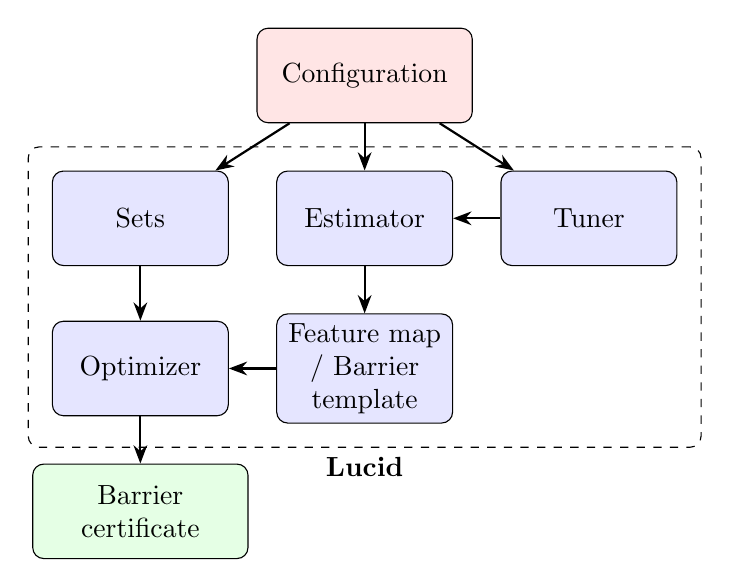
\begin{tikzpicture}[node distance=0.6cm and 0.6cm,
            input-block/.style={rectangle, draw, fill=red!10, text width=2.5cm, minimum height=1.2cm, align=center, rounded corners},
            output-block/.style={rectangle, draw, fill=green!10, text width=2.5cm, minimum height=1.2cm, align=center, rounded corners},
            block/.style={rectangle, draw, fill=blue!10, text width=2.0cm, minimum height=1.2cm, align=center, rounded corners},
            arrow/.style={thick,->,>=Stealth},
            tool/.style={rectangle, draw, fill=magenta!10, text width=3cm, minimum height=0.8cm, align=center, rounded corners},
            inv/.style={}
        ]

        % Input block
        \node[input-block] (input) {Configuration};

        % Lucid blocks
        \node[block, below=of input] (estimator) {Estimator};
        \node[block, right=of estimator] (tuner) {Tuner};
        \node[block, left=of estimator] (sets) {Sets};
        \node[block, below=of estimator] (feature) {Feature map / Barrier template};
        \node[block, left=of feature] (optimizer) {Optimizer};
        % \node[block, below=of optimizer] (verifier) {Verifier};
        \node[draw, dashed, inner sep=0.3cm, rounded corners,
        % fit=(estimator)(feature)(optimizer)(verifier), label=above:{\textbf{Lucid}}] {};
        fit=(estimator)(feature)(optimizer)(sets)(tuner), label=below:{\textbf{Lucid}}] {};

        % Output block
        % \node[output-block, left=of verifier] (output) {Barrier certificate};
        \node[output-block, below=of optimizer] (output) {Barrier certificate};

        % Smt solvers
        % \node[inv, below=2.5cm of verifier.north, anchor=north] (smtInv) {};
        % \node[tool, left=0.3cm of smtInv] (dreal) {dReal};
        % \node[tool, right=0.3cm of smtInv] (cvc5) {CVC5};
        % \node[draw, dashed, inner sep=0.3cm, rounded corners,
        % fit=(dreal)(cvc5), label=left:{\textbf{SMT Solver}}] {};

        % Arrows
        \draw[arrow] (input) -- (estimator);
        \draw[arrow] (input) -- (tuner);
        \draw[arrow] (input) -- (sets);
        \draw[arrow] (sets) -- (optimizer);
        \draw[arrow] (tuner) -- (estimator);
        \draw[arrow] (estimator) -- (feature);
        \draw[arrow] (feature) -- (optimizer);
        % \draw[arrow] (optimizer) -- (verifier);
        % \draw[arrow] (verifier) -- (output);
        \draw[arrow] (optimizer) -- (output);

        % \draw[arrow] (cvc5.north) -- (verifier.south);
        % \draw[arrow] (dreal.north) -- (verifier.south);

    \end{tikzpicture}
    \caption{General architecture of Lucid, highlighting its core components and their connections.}
    \label{fig:architecture}
\end{figure}


\paragraph{\Circled{1}~Safety Specification}
\lucid understands \texttt{RectSet}s and \texttt{Multiset}s, i.e., collections of sets.
These are used to indicate the bounds of the whole state space $\X$, the initial set $\X_0$ and the unsafe set $\X_U$ when defining the safety specification.
They also provide some utility methods for sampling and creating a lattice of the subspaces they define.

\paragraph{\mbox{\Circled{2}\hspace{.4em}Estimator}}
The core of \lucid is its \texttt{KernelRidgeRegressor}\OS{Since the name is exposed, can we call this sth less controversial like KernelRegressor (see also \url{https://en.wikipedia.org/wiki/Kernel_regression}) or simply Estimator. It is easier to use consistent names in Figure~\ref{fig:architecture}.}, which uses a \texttt{GaussianKernel} to learn the underlying system dynamics from the samples.
Its predictions are then used to produce the next state of all the lattice points we need from $\X$, necessary to determine the constraints for the \gls{cbc}.

\paragraph{\Circled{3}~Tuners}
Kernel methods do not require the expensive learning process of other machine learning methods, such as neural networks.
However, they still depend on a number of \hp, such as the kernel bandwidth $\sigma_f$, the lengthscale $\sigma_l$, and the number of Fourier coefficients $M$.
Changes in their values can have a significant impact on the \estimator's efficiency and accuracy.
The process of finding good values for these \hp is known as \emph{hyperparameter tuning}, with the optimal parameters being problem dependent.
\lucid provides a set of utilities, which specialize the \texttt{Tuner} interface, to aid in this task.
{\color{blue}The following tuners are available:
\begin{itemize}
    \item \texttt{MedianHeuristicTuner}: ... (mention that this is restricted to $\sigma_f$ and $\sigma_l$)
    \item \texttt{GridSearchTuner}: ...
    \item \texttt{LBFGSTuner}: ...
\end{itemize}}
\OS{We can also present the 3 different choices as bullets.}
A cheap starting point when working with a Gaussian kernel as in~\eqref{eq:gaussian_kernel} is to use the \emph{median heuristic} \cite{garreau2018largesampleanalysismedian}, implemented in the \texttt{MedianHeuristicTuner}.
\OS{We can cut the following to save space. This is standard knowledge:}
{\color{gray}
We choose $\sigma_l^2$ to be the median of the squared distances between all pairs of points in the training set, i.e.,
\begin{equation}
    \sigma_l^2 = \mathrm{median}_{1 \leq i < j \leq N}\left(\|\hat{x}_i-\hat{x}_j\|^2\right),
\end{equation}
where $\hat{x}_1,\ldots,\hat{x}_N$ are the $N$ training samples.
If $N(N-1)/2$ is even, the median is the average of the two middle values in the sorted list of distances.}
The \texttt{GridSearchTuner}, on the other hand, implements the grid search method, exploring the space of possible \hp values to find the one that yields the best \estimator $R^2$ score,
defined as $R^2 = 1 - \frac{\sum_{i=1}^n (y_i - \hat{y}_i)^2}{\sum_{i=1}^n (y_i - \bar{y})^2}$.
This approach is simple to implement and can be very effective for small problems, but it can become computationally expensive for larger ones.
Borrowing a technique from Gaussian processes, we can also optimize the \hp to maximize the \emph{log marginal likelihood}, defined as
\begin{equation}
    \begin{split}
        &\log p(X^+_N | X_N,\theta) =  - \frac{1}{2}X^+_N{}\T (K_{X}^N + N\lambda I_N)^{-1} X^+_N \\
        &\hspace{40pt} -\frac{1}{2}\log |K_{X}^N + N\lambda I_N| - \frac{N}{2}\log(2\pi),
    \end{split}
\end{equation}
where $\theta:=(\sigma_f,\sigma_l, M)$ \OS{Which are implemented?} contains all learnable hyperparameters (of the kernel).
To do so, the \texttt{LBFGSTuner} uses the L-BFGS or L-BFGS-B quasi-Newton optimization algorithms~\cite{book:nonlinear-programming},
implemented in the \texttt{LBFGS++} library\footnote{https://github.com/yixuan/LBFGSpp}.

\paragraph{\Circled{4}~Feature Map}
We exploit the spectral kernel expansion in \eqref{eq:sqexp_kernel_fourier} by building an explicit approximated feature map, composed of a linear sum of trigonometric functions with increasingly high frequencies.
The full expansion of the kernel would need a sum of infinitely many terms with diminishing impact on the overall result, which we truncate arbitrarily short, a decision based on the tradeoff we are looking for between efficiency and accuracy.
After being defined with the same \hp that characterize the \texttt{KernelRidgeRegressor}, the function can be used to map any point from $\X$ to the \gls{rkhs} defined by the kernel.
\todo{link to the theory} There are currently three different ways the probability distribution can be divided in when associated to the frequency bands as shown in Figure~\ref{fig:spectral_measure_abstraction}:
\begin{itemize}
    \item ...
    \item ...
    \item ...
\end{itemize}
The whole interval can be divided equally, with a logarithmic scale or in smaller intervals with an arbitrary size.
Trying out different feature map implementations may yield different results.

\paragraph{\Circled{5} Solver}
\todo{Barriers should probably be an explicit class in \lucid that hides the opitmisation implementation}
The finite-constraint relaxation of the SIP \eqref{eq:semiinf-prog} is what \lucid uses to synthesize the \gls{cbc} $\B$.
When verifying the safety of a system, \lucid will search for a \gls{cbc} $\B$ that satisfies the conditions in Definition~\ref{def:cbc}.
If it finds it, it will return the constants $\eta$, $\gamma$, and $c$, as well as the \gls{cbc} $\B$ itself, which becomes a certificate of safety for the system $\S$.
More precisely, we follow the steps outlined in~\ref{fig:steps}.
While the theory gives us precise indication on how to construct the \gls{lp} which would yield a correct-by-design solution,
in practice the constraints may prove to be too conservative.
To mitigate this, the user can either increase the number of lattice points $Q$, worsening the computational efficiency,
or adjust the coefficient $C_{\hat{N}}$, improving performance at the cost of loosening the guarantees.
The resulting barrier can then be checked with the verifier, provided we have access to the system's model, to ensure its correctness.
\lucid can be configured to work with any of the following linear optimizers: \gurobi, \alglib or \highs.

\OS{Plot barrier here and give sat. prob.}



\paragraph{Validation (optional)}
Albeit, if \lucid finds a barrier, this is already formally sound with respect to the data-driven estimator, we provide an option to check the validity using an SMT solver.
The solution, if found, will determine the barrier certificate coefficients, as well as the satisfaction probability.
\lucid provides the option to employ the \dreal SMT solver to verify the barrier formally if the system dynamics are known.

\OS{Here just say we know the expected behavior. Thus, via the SMT we get passed}


\subsection{GUI}


\OS{End then end the chapter}

\subsection{Configuration}

The recommended way to use \lucid is through its Python wrapper \pylucid.
After being installed, it can be invoked from the command line with \lstinline|pylucid|.
To define the scenario to run, we suggest using a \yaml or equivalent \json file.
\footnote{The Json schema for \yaml and \json files can be found at \url{https://tendto.github.io/lucid//configuration_schema.json}}\OS{I would personally avoid the word "scenario", as it could be misunderstood with an actual run of the system.}
The same configuration values can also be given to the executable directly as command line arguments.
For a list of all available options, run \lstinline|pylucid --help|.
If more flexibility is needed, a python script can be provided instead,
with the only requirement being that it must contains a function named \lstinline|scenario_config| returning \texttt{Configuration} object.
Any configuration file can be loaded with the command \lstinline|pylucid <config file>|.
\pylucid also provides a \gls{gui} to guide the user in the creation of the scenario configuration and presenting the results in an intuitive way.
To start the \gls{gui}, make sure to have installed the necessary dependencies with \lstinline|pip install pylucid[gui]| \todo{Installation guide?} \Sadegh{Check the level of details provided in the other similar tools papers accepted in the same/similar venue (not control/HSCC, but AI conferences). We can add some basic details here, like a paragraph. Extensive details can go into the appendix, or simply including the user manual as a pdf in the suppelmentary materials.} and run the command \lstinline|pylucid-gui|.
This will open a browser tab containing the interface shown in Figure~\ref{fig:gui}, while a local server will listen for requests coming from the \gls{gui}, computing and returning the results.
\todo{Improve picture of the GUI}
\begin{figure}
    \centering
    \includegraphics[width=\linewidth]{figures/placeholder.jpeg}
    \caption{The GUI of \lucid with the main functions highlighted.}
    \label{fig:gui}
\end{figure}

\subsection{Functionality}

Having parsed and validated the scenario configuration, \lucid will begin the main pipeline to produce the expected result.
If a set of sample transitions has not been provided by the user, \lucid will try to produce it itself by randomly sampling $\X$ to which apply the system dynamics function.
The samples will be used to fit and optionally tune the \estimator so that, given an input state, it will accurately predict the value of the feature map applied to the next state.
\lucid will then store a lattice of points from each of the set provided to which apply the feature map.
These values will be used to define the constraint of the \gls{lp} that the chosen optimizer will solve.


\Sadegh{In the following figure, when you say collect samples, it should be the dataset mentioned earlier in the paper. You also need the next state.}



\section{Example Use Case}
\label{sec:example}

To illustrate \lucid's workflow, we present a simple linear test case.
This example demonstrates how to configure and run the tool to certify the safety of a one-dimensional linear system subject to stochastic noise.\OS{Would it be useful to use this simple example throughout the main text as a running example?}

\paragraph{System Description}
Consider the following discrete-time linear system:
\begin{equation*}
    \begin{bmatrix}
        {x}_{1, t+1}
    \end{bmatrix}
    = \begin{bmatrix}
        0.5
    \end{bmatrix}
    \begin{bmatrix}
        {x}_{1, t}
    \end{bmatrix} + w_t,
    \quad w_t \sim \mathcal{N}(\cdot | 0, 0.01)
\end{equation*}
where $x_t$ is the state at time $t$ and $w_t$ is Gaussian noise.
Given the state space $\X = [-1, 1]$, the goal is to certify that, starting from an initial set $X_0 = [-0.5, 0.5]$, the system avoids the unsafe regions $X_u = [-1, -0.9] \cup [0.9, 1]$ over a finite time horizon.

\paragraph{Configuration via YAML}
We can define the system dynamics, sets, and algorithmic parameters in a YAML configuration file
\lstinputlisting[language=yaml,caption={\texttt{example.yaml} configuration file.}]{code/example.yaml}

We truncate the Fourier expansion to $5$ terms, including the constant term, and use $64$ times the Nyquist frequency of lattice points to build the constraints of the optimization problem, to avoid it being too conservative.
We also provide the \hp values for the kernel, namely the bandwidth $\sigma_f = 1$ and the length scale $\sigma_l = 1.75555556$, values obtained from a previous tuning process.
The user can adjust these values to match their scenario and experiment with different settings.

\paragraph{Configuration via Python}
We can also define the same exact configuration in Python, allowing for more flexibility and programmatic control.
\lstinputlisting[language=iPython,caption={Python configuration for the example.}]{code/example.py}
Note that in this case we are building the \estimator ourself instead of just providing the type of \estimator to use.
This gives us absolute control over how the \estimator is tuned before being used.

\paragraph{Running the Example}
To run the test case, use the command \lstinline|pylucid example.yaml|.
\lucid will parse the configuration, sample the state space and apply the transition function to produce the data used to fit the \estimator, synthesize a barrier certificate, plot and verify the result.
In this case, we are able to obtain a barrier certificate for a time horizon of $T = 15$ which shows a $95.15\%$ satisfaction probability, with $\eta = 0.257, c = 0.031, \|B\| = 1.72$.
The barrier is shown in Figure~\ref{fig:example}.

\begin{figure}
    \centering
    \resizebox{\columnwidth}{!}{\import{figures}{example.pgf}}
    \caption{Barrier certificate for the linear system example. The green line represents the barrier value at time $t$ while the purple one represents the barrier value at time $t+1$.
        The initial and unsafe sets are highlighted in blue and red respectively.}
    \label{fig:example}
\end{figure}

\section{Experimental Evaluation}
\label{sec:experiments}

Platform, configuration, seed

\subsection{Barrier 3}

The first benchmark is inspired by the example \barr from \cite{abate2021fossil}, which we extend by adding stochastic noise $w_t\sim\mathcal{N}(\cdotx\vert 0,0.01I_2)$ to arrive at the two-dimensional nonlinear stochastic dynamics
\begin{equation*}
    \begin{bmatrix}
        {x}_{1, t+1} \\
        {x}_{2, t+1}
    \end{bmatrix}
    = \begin{bmatrix}
        {x}_{2, t} \\
        \frac{1}{3} {x}^3_{1, t} - {x}_{1,t} - {x}_{2,t}
    \end{bmatrix} + w_t.
\end{equation*}
We illustrate the setup in Figure~\ref{fig:CSBarr3}.

The goal is to compute the probability that the system initialized in $[{x}_{1,0},{x}_{2,0}]\T\in \X_0$ (blue regions) does not enter the unsafe regions $\X_U$ (in red) within $T=10$ time steps.

\begin{figure}[ht]
    \resizebox{\columnwidth}{!}{\import{figures}{barrier3.pgf}}%
    \caption{\gls{cbc} synthesis for the \barr benchmark.
        The blue regions represent the initial set $\X_0$, while the red regions represent the unsafe set $\X_U$.
        The pink surface indicates the value of $\gamma$.
    }
    \label{fig:CSBarr3}
\end{figure}

\begin{table}
    \centering
    \begin{tabular}{cccc}
        \toprule
        \textbf{Benchmark} & \textbf{Dim} & \textbf{Runtime} & \textbf{Safety Prob.} \\
                           &              & [m:ss]           & [\%]                  \\ % Units
        \midrule
        Barr3              & 2            & X:XX             & XX                    \\
        name1              & 3            & X:XX             & XX                    \\
        name2              & 7            & X:XX             & XX                    \\
        \bottomrule
    \end{tabular}
    \caption{Computational benchmarks: ...}
    \label{tbl:benchmarks}
\end{table}


Overview of the experimental results in Table~\ref{tbl:benchmarks_results}.
\begin{table}[tb]
    \centering
    \begin{tabular}{ccccc}
        \toprule
        \textbf{Benchmark} & \textbf{Dim} & \textbf{\#LatP} & \textbf{Runtime} & \textbf{Safety Prob.} \\
                           &              &                 & [mm:ss]          & [\%]                  \\ % Units
        \midrule
        Linear             & 1            &                 & X:XX             & XX                    \\
        Barr3              & 2            & $30^2$          & X:XX             & XX                    \\
                           &              & $40^2$          & X:XX             & XX                    \\
        Overtaking         & 3            &                 & X:XX             & XX                    \\
        name2              & 7            &                 & X:XX             & XX                    \\
        \bottomrule
    \end{tabular}
    \caption{Computational benchmarks: ...}
    \label{tbl:benchmarks_results}
\end{table}

\begin{figure}
    \centering
    \includegraphics[width=\linewidth]{placeholder.jpeg}
    \caption{Barrier}
    \label{fig:barr3_barrier}
\end{figure}

\Sadegh{Are we comparing with alternative approaches in the literature? Since we mention alternative tools and their capabilities in Table 1, this raises expectations that we provide a fair benchmarking and show how we are better than them.}

\section{Future Extensions}\label{sec:future_extensions}
The form of data \eqref{eq:data} considered here assumes access to full state measurements, as it is the case when working with simulated systems. Extending this to partially observed settings adds another level of complexity. Extending \lucid to such settings is on our agenda and builds on top of the results presented in this paper.




\section{Conclusion}\label{sec:conclusion}

\OS{Will add some more theoretical details in the appendix, if needed.}
% % !TEX root =  main.tex
\appendix

% \section{Additional Theoretical Details}
% \paragraph{RKHS basics.}
% A symmetric function $k_\X:\X\times\X\rightarrow\R$ is called a (positive definite) \emph{kernel} (note the distinction from \emph{probability kernels}) if for all $N\in\N_{>0}$ we have $\sum_{i=1}^{N}\sum_{j=1}^{N}a_i a_j\allowbreak k_\X(x_i,x_j) \geq 0$ for $x_1,\ldots,x_N\in\X\subset{\R^n}$ and $a_1,\ldots,a_N\in\R$.
% A prominent example is the \emph{squared exponential} (SQExp) kernel \shortcite{Rasmussen2005GP,Kanagawa2018GPvsKernel}:
% \begin{equation}
%     k_\X(x,x') := \sigma_f^2 \exp\left( -\frac{1}{2} (x-x')\T \Sigma\, (x-x') \right),\quad \Sigma:=\mathrm{diag}(\sigma_l)^{-2},\label{eq:sqexp_kernel}
% \end{equation}
% with amplitude $\sigma_f^2\geq0$ and lengthscale coefficients $\sigma_l\in\R^n$.
% \new{For this work,} we assume that all kernels are bounded on their domain, i.e., $\E_{}[k_\X(x,x)]<\infty$, $x\in\X$.
% Given a kernel $k_\X$ on a non-empty set $\X$, there exists a unique corresponding
% \emph{reproducing kernel Hilbert space} (RKHS) $\Hilbert_{k_\X}$
% of functions $f:\X\rightarrow\R$ equipped with an inner product $\innerH{\cdotx}{\cdotx}{\Hilbert_{k_\X}}$
% with the celebrated \emph{reproducing property} such that for any function $f\in\Hilbert_{k_\X}$ and $x\in\X$ we have $f(x)=\innerH{f}{k_\X(\cdotx,x)}{\Hilbert_{k_\X}}$.
% Note that $k_\X(\cdotx,x):\X\rightarrow\Hilbert_{k_\X}$ is a real-valued function,
% which is also called an implicit \emph{canonical} \emph{embedding} or \emph{feature map} $\phi_\X$
% such that $k_\X(x,x')=\innerH{\phi_\X(x)}{\phi_\X(x')}{\Hilbert_{k_\X}}$ for all $x,x'\in\X$.
% For an RKHS $\Hilbert_{k_\X}$, we use the associated feature map $\phi_\X$ and kernel $k_\X$ interchangeably for ease of notation and comprehensibility.
% The inner product induces the norm $\norm{f}_{\Hilbert_{k_\X}}\!\!\!\!:=\!\!\sqrt{\smash[b]{\innerH{f}{f}{\Hilbert_{k_\X}}}}$ of the RKHS. 
% Throughout this paper, we assume that all RKHSs are \emph{separable}.
% Refer to the monograph by \citet{Berlinet2004RKHSProbStat} for a comprehensive study on RKHSs.
% Given $N$ i.i.d. samples $\hat X_N:=[\hat{x}_i]_{i=1}^N$ with $\hat{x}_i\in\X$, the
% \emph{Gram matrix} of $k_\X$ is given by
% $\new{K_{\hat{X}}^N}:=[k_\X(\hat{x}_i,\hat{x}_j)]_{i,j=1}^N.$
% Furthermore, we define the vector-valued function 
% $\new{k_{\hat{X}}^N}(x)  := [k_\X(x,\hat{x}_i)]_{i=1}^N.$

% \begin{definition}[Conditional Mean Embedding (CME)]\label{def:condMeanEmbed}
%     Given two RKHSs $\Hilbert_{k_\X}$ and $\Hilbert_{k_\Y}$ with the associated kernels $k_\X\colon\X\times\X\to\R$ and $k_\Y\colon\X\times\X\to\R$, the \emph{CME} of a probability kernel $\Tr\colon\X\times\borel{\Y}\rightarrow[0,1]$ is an $X$-measurable random variable taking values in $\Hilbert_{k_\Y}$, given by
%     \begin{equation*}
%         \cme_{k_\Y|k_\X}(\Tr)(\cdotx) := \E_{\Tr}[\phi_\Y(Y)\mid X=\cdotx].
%     \end{equation*}
% \end{definition}

\section{Linear Program}
The finitely-constrained LP discussed in Section~\ref{sec:ddbarriers} is presented. For this, the lattices $X_{{N}}\subset\X$, $\smash{\{ x_0^{1}, \ldots, x_0^{{N}_0} \}} \subset \X_0$, and $\smash{\{ x_u^{1}, \ldots, x_u^{{N}_u} \}} \subset \X_u$ of cardinality ${N}_0\in\N$ and ${N}_u\in\N$, respectively, are formed.
%
For given values of $\overline{\B}$, $\gamma$, and robustness radius $\mathcal{R}\geq0$, the following LP is obtained:
\begin{equation*}
      \begin{alignedat}{3}
                  & \min_{\stackrel{b, c, \eta}{\Bmin_{{N}}^{\X_0}, \Bmax_{{N}}^{\X_u},\Bmax_{{N}}^\X,\Bmin_\Delta}}\hspace{-1.5em} &                                          & \eta + cT,                                    &                   &
            %\label{eq:blackbox:linear_prog_objective}
            \\
                  & \text{subject to}
                  &                                                                                                                 & \phi_M(x_0^{i})\T b\leq\hat{\eta}, \quad &                                               & i=1,\ldots,{N}_0,
            %\label{eq:blackbox:linear_prog_initial}
            \\
                  &                                                                                                                 &                                          & \phi_M(x_u^{i})\T b\geq\hat{\gamma},
            \quad &                                                                                                                 & i=1,\ldots,{N}_u,
            %\label{eq:blackbox:linear_prog_unsafe}
            \\
                  &                                                                                                                 &                                          & \phi_M(x^{i})\T(Hb - b) \leq \hat{\Delta},
            \quad &                                                                                                                 & i=1,\ldots,{N},
            %\label{eq:blackbox:linear_prog_kushner}
            \\
                  &                                                                                                                 &                                          & \phi_M(x^{i})\T b\geq \hat{\xi},
            \quad &                                                                                                                 & i=1,\ldots,{N},
            %\label{eq:blackbox:linear_prog_positive}
            \\
                  &                                                                                                                 &                                          & \Bmin_{{N}}^{\X_0}\leq\phi_M(x_0^{i})\T b,
            \quad &                                                                                                                 & i=1,\ldots,{N}_0,                                                                                              \\
                  &                                                                                                                 &                                          & \Bmax_{{N}}^{\X_u}\geq\phi_M(x_u^{i})\T b,
            \quad &                                                                                                                 & i=1,\ldots,{N}_u,                                                                                              \\
                  &                                                                                                                 &                                          & \Bmax_{{N}}^\X\geq\phi_M(x^{i})\T b,
            \quad &                                                                                                                 & i=1,\ldots,{N},                                                                                                \\
                  &                                                                                                                 &                                          & \Bmin_\Delta\leq\phi_M(x^{i})\T (Hb - b),
            \quad &                                                                                                                 & i=1,\ldots,{N},                                                                                                \\
                  &                                                                                                                 &                                          & c\geq 0,\,\gamma>\eta\geq 0,\, b\in\R^{2M+1}, &                   &
            \label{eq:blackbox:linear_prog}%
      \end{alignedat}
\end{equation*}
with $\overline{\kappa}\geq\sigma_f$, $\overline{\B}\geq\norm{b}_2$, and constraint-tightening coefficients
\begin{align*}
      \hat{\eta}   & := \frac{2}{C_{{N}}+1}\eta + \frac{C_{{N}}-1}{C_{{N}}+1}\Bmin_{{N}}^{\X_0},
      \\                                                                                                                                    & \hat{\gamma} := \frac{2}{C_{{N}}+1}\gamma + \frac{C_{{N}}-1}{C_{{N}}+1}\Bmax_{{N}}^{\X_u}, \\
      \hat{\Delta} & := \frac{2}{C_{{N}}+1}\left(c - \mathcal{R}\overline{\B}\overline{\kappa}\right) + \frac{C_{{N}}-1}{C_{{N}}+1}\Bmin_\Delta,
      \\                                                                                                                                     & \hat{\xi} := \frac{C_{{N}}-1}{C_{{N}}+1}\Bmax_{{N}}^\X.
\end{align*}


% \section{Proofs}
% We have collected a series of proofs of the claims we made in the main text.

\section{Installation}
Provided \texttt{Python>=3.8} is already present, \pylucid can be installed with the command
\begin{lstlisting}[language=bash,numbers=none,xleftmargin=0em]
pip install pylucid[gui,plot] --index-url \
  https://gitlab.com/api/v4/projects/71977529/packages/pypi/simple
\end{lstlisting}
There are a few limitation some of the dependencies introduce, which may preclude the ability of using certain features on not supported platforms.
Formal verification of the barrier requires the \dreal SMT solver, which can only be installed on Linux and non-ARM macOS.
Support for \highs \gls{lp} is not available on Windows at the moment.
The \gurobi solver must be installed beforehand, and requires a license for commercial use, but is free for academic purposes.

For more details on the installation process, please refer to the online documentation at \url{https://lucidtoolsource.gitlab.io/lucid/md_docs_2Pylucid.html}.

\section{Benchmarks}
\label{app:benchmarks}
Complete list of results for the benchmarks presented in Section~\ref{sec:experiments}.
The legend is as follows:
\textit{Output} indicates the result produced by the solver (i.e., optimal, unbounded, infeasible or unspecified),
\textit{Prec} indicates the number of bits used in the last floating-point number representation,
\textit{Ref} indicates the number of refinements,
and \textit{time} is the time in seconds.

All benchmarks were run on a Windows 10 machine with an AMD Ryzen 9 5950X 16-Core Processor @ 3.40 GHz, and 64 GB of RAM, and all runs had the random seed set to $42$ to ensure reproducibility.
The scripts responsible for running the benchmarks and \hp tuning are available in the \texttt{benchmarks/integration} folder of the repository.
Note that a version of \texttt{Python>=3.9} is required to run the scripts, as some dependencies used to track the benchmarks' metrics across multiple runs are not compatible with \texttt{Python 3.8}.
The \hp tuning of the \estimator was performed with the \texttt{LbfgsTuner}, bounding the value of $\sigma_l$ between $[10^{-5}, 10^5]$, and refined with the \texttt{GridSearchTuner}.
The implementation can be found in the \texttt{benchmarks/integration/hp\_tuning.py} script. 
Note that we used the \gurobi optimiser.
Other optimizers, such as \alglib or \highs, can be used instead, but may yield different results, especially in terms of performance.

\subsection{Linear}

We consider the following system:
\begin{equation*}
    \begin{bmatrix}
        {x}_{t+1}
    \end{bmatrix}
    = \begin{bmatrix}
        0.5 {x}_{t}
    \end{bmatrix} + w_t,
\end{equation*}
where $w_t\sim\mathcal{N}(\cdotx\vert 0,0.01I_1)$.
Given
\begin{align*}
    &\X = [-1, 1] \\
    &\X_0 = [-0.5, 0.5] \\
    &\X_U = [-1, -0.9] \cup [0.9, 1],
\end{align*}
we want to ensure that the system, starting in $\X_0$, does not enter the unsafe regions $\X_U$ within $T=15$ time steps.
The complete configuration for the linear example benchmark is shown in Listing~\ref{lst:linear}.
\lstinputlisting[language=yaml,caption={Configuration for linear example},captionpos=b,label={lst:linear}]{code/linear.yaml}

\subsection{Barrier 2}

We consider the following system:
\begin{equation*}
    \begin{bmatrix}
        {x}_{1, t+1} \\
        {x}_{2, t+1}
    \end{bmatrix}
    = \begin{bmatrix}
        {x}_{2, t} - 1 + e^{-x_{1, t}} \\
        -\sin^2(x_{1, t})
    \end{bmatrix} + w_t,
\end{equation*}
where $w_t\sim\mathcal{N}(\cdotx\vert 0,0.01I_2)$.
Given
\begin{align*}
    &\X = [ -2, 2 ] \times [ -2 , 2 ] \\
    &\X_0 = \{ [x_1, x_2] : (x_1 + 0.5)^2 + (x_2 - 0.5)^2 \leq 0.4 \} \\
    &\X_U = \{ [x_1, x_2] : (x_1 - 0.7)^2 + (x_2 + 0.7)^2 \leq 0.3 \},
\end{align*}
we want to ensure that the system, starting in $\X_0$, does not enter the unsafe regions $\X_U$ within $T=5$ time steps.
The complete configuration for the \barrII benchmark is shown in Listing~\ref{lst:barrier2}.
\lstinputlisting[language=yaml,caption={Configuration for \barrII},captionpos=b,label={lst:barrier2}]{code/barrier2.yaml}

\subsection{Barrier 3}

We consider the following system:
\begin{equation*}
    \begin{bmatrix}
        {x}_{1, t+1} \\
        {x}_{2, t+1}
    \end{bmatrix}
    = \begin{bmatrix}
        {x}_{2, t} \\
        \frac{1}{3} {x}^3_{1, t} - {x}_{1,t} - {x}_{2,t}
    \end{bmatrix} + w_t,
\end{equation*}
where $w_t\sim\mathcal{N}(\cdotx\vert 0,0.01I_2)$.
Given
\begin{align*}
    &\X = [ -3, 2.5 ] \times [ -2 , 1 ] \\
    &\X_0 = [ 1 , 2 ] \times [ -0.7 , 0.3 ] \cup [ -1.8 , -1.4 ] \times [ -0.1 , 0.1 ] \\
    &\qquad \cup [-1.4, -1.2] \times [-0.5 , 0.1] \\
    &\X_U = [ 0.4 , 0.6 ] \times [ 0.2 , 0.6 ] \cup [ 0.6 , 0.7 ] \times [ 0.2 , 0.4 ],
\end{align*}
we want to ensure that the system, starting in $\X_0$, does not enter the unsafe regions $\X_U$ within $T=5$ time steps.
The complete configuration for the \barrIII benchmark is shown in Listing~\ref{lst:barrier3}.
\lstinputlisting[language=yaml,caption={Configuration for \barrIII},captionpos=b,label={lst:barrier3}]{code/barrier3.yaml}

\subsection{Overtaking}

We consider a scenario where an autonomous vehicle (AV) controlled by a \gls{nn} is overtaking another vehicle.
The dynamics of the ego vehicle are given by Dubin's car model \EC{does it need a cit or is it just textbook} by adding the noise vector $w = \begin{bmatrix}w_t^1 & w_t^2 & w_t^3\end{bmatrix}$ where each component is drawn from a zero-mean Gaussian with standard deviation $0.01$, $0.01$, and $0.001$, respectively.
The steering wheel angle is supplied by the \gls{nn} controller and we travel at a fixed velocity $v=1$.
Given
\todo{correct the sets}
\begin{align*}
    &\X = [ -3, 2.5 ] \times [ -2 , 1 ] \\
    &\X_0 = [ 1 , 2 ] \times [ -0.7 , 0.3 ] \cup [ -1.8 , -1.4 ] \times [ -0.1 , 0.1 ] \\
    &\qquad \cup [-1.4, -1.2] \times [-0.5 , 0.1] \\
    &\X_U = [ 0.4 , 0.6 ] \times [ 0.2 , 0.6 ] \cup [ 0.6 , 0.7 ] \times [ 0.2 , 0.4 ],
\end{align*}
we want to ensure that the system, starting in $\X_0$, does not enter the unsafe regions $\X_U$ within $T=5$ time steps.

The complete configuration for the \overtaking benchmark is shown in Listing~\ref{lst:overtaking}.
\lstinputlisting[language=yaml,caption={Configuration for \overtaking},captionpos=b,label={lst:overtaking}]{code/overtaking.yaml}



%%%%%%%%%%%%%%%%%%%%%%%%%%%%%%%%%%%%%%%%%%%%
%%%%%%%%%%%%%%%%%%%%%%%%%%%%%%%%%%%%%%%%%%%%
%%%%%%%%%%%%%%%%%%%%%%%%%%%%%%%%%%%%%%%%%%%%
\bibliography{aaai25}

\end{document}
